\section{Reproducibility Summary}

\subsection*{Scope of Reproducibility}

This report covers our reproduction and extension of the paper `When Does Self-Supervision Improve Few-shot Learning?' published in ECCV 2020. The paper investigates the effectiveness of applying self-supervised learning (SSL) as a regularizer to meta-learning based few-shot learners. The authors of the original paper claim that SSL tasks reduce the relative error of few-shot learners by 4\% - 27\% on both small-scale and large-scale datasets, and the improvements are greater when the amount of supervision is lesser, or when the data is noisy or of low resolution. Further, they observe that incorporating unlabelled images from other domains for SSL can hurt the performance of FSL, and propose a simple algorithm to select unlabelled images for SSL from other domains to provide improvements. 

\subsection*{Methodology}

We conduct our experiments on an extended version of the authors codebase. We implement the domain selection algorithm from scratch. We add datasets and methods to evaluate few-shot learners on a cross-domain inference setup. Finally, we open-source pre-processed versions of $3$ few-shot learning datasets, to facilitate their off-the-shelf usage. We conduct experiments involving combinations of supervised and self-supervised learning on multiple datasets, on 2 different architectures and perform extensive hyperparameter sweeps to test the claim. We used 4 GTX 1080Ti GPUs throughout, and all our experiments including the sweeps took a total compute time of 980 GPU hours. Our codebase is at \href{https://github.com/ashok-arjun/MLRC-2021-Few-Shot-Learning-And-Self-Supervision}{https://github.com/ashok-arjun/MLRC-2021-Few-Shot-Learning-And-Self-Supervision}.
\subsection*{Results}

On the ResNet-18 architecture and a high input resolution that the paper uses throughout, our results on 6 datasets overall verify the claim that SSL regularizes few-shot learners and provides higher gains with difficult tasks. Further, our results also verify that out-of-distribution images for SSL hurt the accuracy, and the domain selection algorithm that we implement from scratch also verifies the paper's claim that the algorithm can choose images from a large pool of unlabelled images from other domains, and improve the performance.

Going beyond the original paper, we also conduct SSL experiments on 5 datasets with the Conv-4-64 architecture with a lower image resolution. Here, we find that self-supervision {does not} help boost the accuracy of few-shot learners in this setup. Further, we also show results on a practical real-world benchmark on \textit{cross-domain few-shot learning}, and show that using self-supervision when training the base models degrades performance when evaluated on these tasks.

\subsection*{What was easy}

The paper was well written and easy to follow, and provided clear descriptions of the experiments, including the hyperparameters. The authors' code implementation in PyTorch was relatively easy to understand.

\subsection*{What was difficult}

Since the codebase was incomplete, it took us a lot of time to solve bugs, and reimplement algorithms not present in the code. Further, the datasets needed a lot of preprocessing to be used. The number of hyperparameters being too many but each proving to be important, and evaluating all the claims of the paper on 5 datasets and 2 architectures was difficult to the number of experiment configurations, resulting in a very high computational cost of 980 GPU hours.

\subsection*{Communication with original authors}

We maintained contact with the authors throughout the challenge to clarify implementation details and questions regarding the domain selection algorithm. The authors were responsive and replied promptly with detailed explanations.

\clearpage

\section{Content}

\section{Scope of reproducibility}
\label{sec:claims}

The paper claims that 

\begin{itemize}
    \item With \textit{no additional training data}, adding self-supervised tasks such as jigsaw/rotation prediction as an auxiliary task improves the performance of existing few-shot techniques on benchmarks across several different domains
    \item The benefits of self-supervision \textit{increase} with the difficulty of the task, for example when training with a base dataset with less labelled data, or when the dataset contains images of lesser quality/resolution
    \item Using unlabelled data from dissimilar domains for self-supervision negatively impacts the performance of few-shot learners
    \item The proposed domain selection algorithm can alleviate this issue by learning to pick images that are similar to the training domain, from a large and generic pool of images 
\end{itemize}

We thoroughly reproduce all the experiments, and investigate whether the claims hold true, with the model and the six benchmark datasets  used by the authors. Beyond the paper, we find that the results are biased towards the architecture and resolution used, and demonstrate that the gains do not hold when the input resolution and architecture differ from those reported in the paper. We also report results on the more practical cross-domain few-shot learning setup. Here, we find that self-supervision \textit{does not} help ImageNet-trained few-shot learners generalize to new domains better. Finally, along with our reproducible codebase, we open-source processed versions of $3$ datasets that previously required tedious manual processing, to facilitate their off-the-shelf usage.

\section{Methodology}

% 1. Protonet, jigsaw, rotation and equation
% 2. Domain selection algorithm

The goal of a few-shot learner is to learn representations of base classes that lead to good generalization on novel classes. To this end, the proposed framework combines \textit{meta learning} approaches for few-shot learning with \textit{self-supervised learning}. In general, learning consists of estimating functions $f$, the feature extractor and $g$, the classifier that minimize the empirical loss $\ell$ over the training data from base class $D_{s} = {\{(x_i, y_i})\}_{i=1}^{n}$ consisting of images $x_i \in \mathcal{X}$ and labels $y_i \in \mathcal{Y}$, along with suitable regularization $\mathcal{R}$. This can be written as:

$$L_s = \sum_{(x_i, y_i) \in D_s^{}} \ell(g \circ f(x_i), y_i)  + \mathcal{R}(f,g)$$

In the original paper, the loss of prototypical networks (ProtoNet)\cite{protonets} are used as part of the supervised loss. During meta-training, ProtoNet computes the mean of the embeddings of all samples in a class. Then, a distance metric such as Euclidean distance or cosine distance is used to classify every query sample into one of the classes, using the distance from the class-prototypes. The loss over the query samples is backpropagated to the network, and this procedure is repeated for multiple episodes with $n$ randomly sampled classes in each episode, with $k$ examples in each class, hence referred to as the n-way k-shot setup. Hence the network meta-learns to provide useful class-prototypes from very few examples. At meta-test time, class prototypes are recomputed from the few examples per each class, and query examples are classified based on the distances to the class prototypes.

Apart from the supervised losses, the paper uses self-supervised losses $\ell_{ss}$ that are derived from $(\hat{x}, \hat{y})$. Let $h$ denote an additional auxiliary classifier used as part of a self-supervised loss, and $D_{ss}$ denote the dataset used to construct the self-supervised tasks. Then the self-supervised loss is 

$$L_{ss} = \sum_{(x_i) \in D_{ss}^{}} \ell(h \circ f(\hat{x_i}), \hat{y_i})$$

The \textit{jigsaw} task splits an image into 9 regions (3x3) and permutes the regions to obtain the input $\hat{x}$. The target label $\hat{y}$ is the index of the permuatation. The total number of indices are $9!$ which is reduced to $35$ indices \cite{noroozi2016unsupervised} by grouping the possible permutations to control the difficulty of the task.

The \textit{rotation} task rotates the image by an angle $\theta \in {0^{\circ}, 90^{\circ}, 180^{\circ}, 270^{\circ}}$ to obtain $\hat{x}$, with $\hat{y}$ being the index of the angle.

The paper uses a weighted combination of the supervised and self-supervised losses $L = (1-\alpha)*L_s + (\alpha)*L_{ss}$. 

The author also propose an algorithm to select images from a large-dataset for self-supervision when $D_s$ and $D_{ss}$ are different. Here, a classifier is trained to distinguish the ResNet-101 features of images from $D_s$ and images from $D_{ss}$, and the top-$k$ images according to the ratio $p(x \in D_s) / p(x \in D_p)$ are selected for self-supervision. 

\section{Experimental settings}

\subsection{Details regarding the code}

The authors provide a public implementation of the code\footnote[1]{\url{https://github.com/cvl-umass/fsl\_ssl}}, which is built upon a popular codebase \footnote[2]{\url{https://github.com/wyharveychen/CloserLookFewShot}} from Chen et al \cite{chen2018a}. We find that there are a lot of errors and bugs in the code, which took a lot of time to debug. This took up a considerable part of  our time. Further, the code for the domain selection algorithm was not present, and hence we had to \textit{reimplement it from scratch}. Our code \footnote[3]{\url{https://github.com/ashok-arjun/MLRC-2021-Few-Shot-Learning-And-Self-Supervision}} reuses multiple files from the original codebase, corrects several errors, and provides an implementation of the domain selection algorithm. We also provide interfaces to train models with a different architecture, and to evaluate models in a cross-domain setup.

\subsection{Model descriptions}

The authors use a well-known architecture ResNet-18 for their experiments. The ResNet18 gives a 512-dimensional feature for each input. For the jigsaw task, a single fully-connected (fc) layer with 512-units is added in parallel to the classifier. Nine patches of an image give nine 512-dimensional feature vectors, which are concatenated, and projected to 4096 dimensions using an fc layer, and then to a 35-dimensional output using another fc layer, corresponding to the 35 permutations for the jigsaw task. 

For rotation prediction task, the 512-dimensional output of ResNet-18 is passed through three fc layers consecutively with {128, 128, 4} units. The 4 predictions of the last layer correspond to the four rotation angles. Between each fc layer, a ReLU activation and a dropout layer with a dropout probability of 0.5 are added.

Apart from the ResNet-18 architecture used in the paper, we use another architecture that is equally adapted in many few-shot learning papers \cite{chen2018a} \cite{protonets} \cite{sung2018learning} \cite{finn2017model}, the Conv-4-64 architecture, which is a simpler architecture with 3x3 kernel size and 64 filters at each layer. Similar extensions are made for the jigsaw and rotation tasks. In multiple works in the literature, this architecture has been used to process $84$ x $84$ images, while the ResNet variants have been used to process $224$ x $224$ images. We follow the works and report results with the respective resolutions for each architecture. Both the architectures are represented diagrammatically in tables \ref{table:conv_arch} and \ref{table:resnet_arch} respectively in the appendix.

\subsection{Datasets}

Following the few-shot setup, each dataset is split into three disjoint sets namely the base training set, validation set and the test set. The model is trained on the \textit{base} set, validated on the \textit{validation} set, and tested on the \textit{test} set.
Following the paper, we experiment with multiple datasets across diverse domains and denote the number of classes in the \textit{base, val, test} splits inside brackets: CUB-200-2011 \cite{cub}(64, 12, 20) , Stanford Cars \cite{cars} (98, 49, 49), FGVC-Aircraft \cite{aircrafts} (50, 25, 25), Stanford Dogs \cite{dogs} (60, 30, 30), Oxford Flowers \cite{flowers} (51, 26, 26). These 5 datasets are henceforth referred to as "the smaller datasets". Apart from these, we also experiment with a benchmark dataset for few-shot learning, the miniImageNet dataset \cite{mini} (64, 16, 20). The original paper also reports results on Tiered-ImageNet, but we restrict to evaluating on miniImageNet due to compute and time constraints. 

We use the same base-validation-novel class splits for every dataset exactly as in the paper, which they provide in their official repository. Implementation-wise, each class contains $3$ files, one for each in base, val and novel, and lists the classes to be used, along with all the image paths for each class.

Among the small datasets, we found that there were no versions of the flowers and cars dataset that could be used directly. Hence we had to preprocess the two datasets ourselves, before we could use them off-the-shelf. With the miniImageNet dataset, we found that all the directly-downloadable versions \cite{rengithub} \cite{yao2github} contained images resized to 84x84, however we needed a dataset that could be resized to either 84x84 or 224x224 adaptively. Hence, we had to download the ImageNet dataset (155 GB) and process the dataset from scratch, which caused storage issues and also took up a significant part of our time. Along with codebase, we also open-source the processed flowers\footnote[4]{\url{https://www.kaggle.com/arjun2000ashok/vggflowers/}} and cars\footnote[5]{\url{https://www.kaggle.com/hassiahk/stanford-cars-dataset-full}} datasets, and the miniImageNet dataset with image sizes same as that in ImageNet\footnote[6]{\url{https://www.kaggle.com/arjunashok33/miniimagenet}}. 

For the domain selection algorithm, the authors use the training sets of two large datasets - Open Images v5 \cite{openimages} and iNaturalist \cite{inat}, which are 500 GB and 200 GB in size respectively. We use the \textit{validation} splits of these datasets as unlabelled images for self-supervision.

\subsection{Hyperparameters}

The hyperparameter sweeps were conducted using Weights and Biases.  Each sweep uses {random search} to search over the following $3$ hyperparameters:

\begin{itemize}
    \item \textbf{Learning Rate}: Sampled from a uniform distribution $(0.0001, 0.03)$
    \item \textbf{Batch normalization mode}: 
    \begin{enumerate}
        \item Use batch normalization, accumulate statistics throughout training, and use the statistics during testing
        \item Use batch normalization, but do not track the running mean and variance during training; estimate them from batches during training and test
        \item No batch normalization
    \end{enumerate}
    \item \textbf{Alpha ($\alpha$)}, the weightage of the SSL term in the loss (only where self-supervision is applied)
\end{itemize}

In the above grid, the batch-norm modes especially designed to verify the claim of the paper that using batch norm mode $2$ was found to be better for a subset of tasks that did not involve jigsaw, and vice-versa. All models are trained with the Adam optimizer with $\beta_1 = 0.9$ and $\beta_2 = 0.999$.

We then use the configuration which gives the best \textit{validation accuracy}. Due to computational constraints, we search hyperparameters for certain datasets, and reuse the hyperparameters found for similar datasets. The selected experiment configurations are given in the appendix and the code-base. Across all of our sweeps, we notice that $\alpha$ stays below $0.6$, and does not go below $0.3$ in our runs. Hence, we infer that an adequate amount of supervision is also needed for good performance, and too much self-supervision hurts accuracy. For the miniImageNet dataset, we find the values close $0.3$ work the best, which the paper reiterates. The paper reports that they use $0.5$ for all the SSL experiments on the small datasets, which we confirm as our $\alpha$ term converges to values $0.4$ and $0.6$ for the small datasets. All of our reported results are with the best hyperparameters found.

\subsection{Computational requirements}
\label{ss:comp_req}

We used 4 Nvidia 1080Ti GPUs for all experiments. The run-times differ for each experiment configuration when incorporating self-supervision. We report the average epoch time for each experimental setup (1 epoch = 100 episodes) in table \ref{table:epoch_time} in the appendix.  

In general, among experiments involving self-supervised learning, rotation took the maximum amount of time. This is because $4$ rotations of the same image are needed at every instance, which is more expensive than loading a single image. The jigsaw task took lesser time than rotation, and the combination of jigsaw and rotation took the highest amount of time per epoch. Since the paper reports results on the combination only for the first set of experiments (claim $1$), we also do the same. Further, the computational time restricted us from performing more experiments combining the two.

In total, apart from the hyper-parameter sweeps, we perform \textbf{250 experiments}, across different experimental setups and multiple datasets. All of these experiments took approximately \textbf{700 GPU hours}. Along with the hyperparameter sweeps which, the experiments took approximately \textbf{980 hours} of compute time. 

\subsection{Experimental setup and code}

Following the authors, we train, evaluate and report results on the 5-way 5-shot setting; we also explore 20-way 5-shot setting but we could not continue after a few runs, restricted by the large training and testing time of 20-way 5-shot models. Following the paper, we use 16 query examples to evaluate the models.

The batch size cannot be set in episodic few-shot learners, and are by default given by $n\_way * (n\_support + n\_query)$. We use 16 query images following the paper, and as a result, our batch sizes are $105$ in 5-way 5-shot experiments, and $420$ in 20-way 5-shot experiments. Following all previous work in few-shot learning, we sample 100 episodes (batches) per epoch, and conduct experiments on about 600 - 800 epochs. Following the paper, we use only 5 query images when training models for experiments that use lesser labelled data since the \{20, 40, 60, 80\}\% splits of dataset do not contain 16 query images in all classes.

In every iteration, an equal number of unlabelled images are sampled at random from the respective dataset(s) for self-supervised learning. Following our paper and the baseline from previous work \cite{chen2018a} in few-shot learning and our original paper, we use the following data augmentation:  For label and rotation predictions, images are first resized to 224 pixels for the shorter edge while maintaining aspect ratio, from which a central crop of 224 is obtained. For jigsaw puzzles, a random crop of 255 is done from the original image with random scaling between [0.5, 1.0], then split into 3×3 regions, from which a random crop of size 64×64 is picked. For evaluation at meta-test time, we use 600 randomly sampled episodes, and report the mean accuracy and 95\% confidence intervals. 

We implement the domain selection algorithm following the paper: For each dataset among the small datasets, we select negative images uniformly at random with 10 times the size of the positive images. The loss for the positive class is scaled by the inverse of its frequency to account for the significantly larger number of negative examples. We then train a binary logistic regression classifier using LBFGS for 10000 iterations and use the logits to compute the ratio $p(x \in D_s) / p(x \in D_p)$, where $D_p$ represents the large pool of images, and $D_s$ represents the supervised training set. We then choose $k$ as 80\% of the total dataset size, and sample $k$ images from the negative class ($D_p$) to use as unlabelled samples.

On verifying that the core claim of the paper (claim $1$) for all the 5 small datasets, we choose a diverse set of $2$ to $3$ representative datasets for claims $2$ and $3$. For the domain selection, we evaluate on all the 5 datasets to verify our implementation of the algorithm.

\section{Results}
\label{sec:results}
\subsection{Results reproducing original paper}
Here, we consider the same architecture that the paper uses - ResNet-18, with an input image size of $224$.
\subsubsection{Self-supervision improves few-shot learning}
Here, we successfully verify claim $1$ of the paper which states that with no additional unlabelled data, SSL improves few-shot learning when applied as an auxiliary task. We conduct experiments across all the 5 small datasets as well as the large-scale miniImageNet dataset. We also reproduce results on the baseline from \cite{chen2018a}, and MAML and MAML+Jigsaw. We present results in figure \ref{fig:Res-18-small}, and tables \ref{table:mini_imagenet} and \ref{table:resnet_few_shot}. All results are on 5-way 5-shot classification.

\begin{table}
	\begin{minipage}{0.55\linewidth}
		\centering
		\includegraphics[height=8.0cm, width=8.5cm]{pdfs/Res18.pdf}
		\captionof{figure}{Results on applying SSL tasks to Prototypical networks, across 6 datasets}
		\label{fig:Res-18-small}
	\end{minipage}\hfill
	\begin{minipage}{0.5\linewidth}
		\centering
		\begin{tabular}{|c|c|c|}
            \hline
            Method & Accuracy \\
            \hline\hline
            ProtoNet & 74.07 \textpm\ 0.71  \\
            ProtoNet + Jigsaw & \textbf{77.29 \textpm\ 0.73}  \\
            ProtoNet + Rotation & 74.93 \textpm\ 0.9  \\
            ProtoNet + Jigsaw + Rotation & 76.23 \textpm\ 0.9  \\
            \hline
        \end{tabular}
        \caption{miniImageNet Results with ResNet-18}
        \label{table:mini_imagenet}
	\end{minipage}
\end{table}

\begin{table*}[hbt!]
\begin{center}
\begin{tabular}{|c|c|c|c|c|c|}
\hline
Method & CUB & Cars & Aircrafts & Dogs & Flowers \\
\hline\hline
Softmax & 81.92 \textpm\ 0.54 & 88.16 \textpm\ 0.47 & 89.57 \textpm\ 0.38 & 78.18 \textpm\ 0.56 & 90.44 \textpm\ 0.47 \\
Softmax + Jigsaw & 83.96 \textpm\ 0.52 & 91.2 \textpm\ 0.49 & 89.93 \textpm\ 0.39 & 78.3 \textpm\ 0.57 & 90.85 \textpm\ 0.49 \\
ProtoNet & 87.09 \textpm\ 0.48 & 91.0 \textpm\ 0.41 & \textbf{91.90 \textpm\ 0.35} & 83.52 \textpm\ 0.54 & 89.92 \textpm\ 0.51 \\
ProtoNet + Jigsaw & \textbf{89.57 \textpm\ 0.43} & 92.67 \textpm\ 0.39 & 91.72 \textpm\ 0.39 & \textbf{86.1 \textpm\ 0.51} & \textbf{90.98 \textpm\ 0.47} \\
ProtoNet + Rotation & 88.9 \textpm\ 0.55 & 91.61 \textpm\ 0.40 & 91.69 \textpm\ 0.40 & 83.94 \textpm\ 0.58 & 90.12 \textpm\ 0.5 \\
ProtoNet + Jigsaw + Rotation & 88.98 \textpm\ 0.45 & \textbf{93.27 \textpm\ 0.38} & 91.26 \textpm\ 0.4 & 85.29 \textpm\ 0.54 & 90.01 \textpm\ 0.51 \\
\hline
\end{tabular}
\end{center}
\caption{ResNet-18's performance on the $5$ small datasets.}
\label{table:resnet_few_shot}
\end{table*}

\subsubsection{The benefits of self-supervision increase with the difficulty of the task}

We successfully verify claim $2$ of the authors that the relative gains of using SSL are more when the difficulty of the task is higher. The authors experiment with two types of difficult tasks: one with low-resolution/greyscale images as input, and another with less labelled data from the base training set. We experiment with $3$ selected datasets and were successful in reproducing the results. We report the results on figures \ref{fig:20-40-60-80} and \ref{fig:lowres}. The exact numbers are given on tables \ref{table:grey_low_res} and \ref{table:20_ssl} respectively in the appendix. We find that the claims of the paper hold true, and that self-supervision has higher gains in harder tasks.

\begin{figure}[t]
    \begin{minipage}{0.33\textwidth}
        % \centering
        \vspace{0.2cm}
        \includegraphics[width=5cm, height=5.5cm]{pdfs/ssl.pdf} % first figure itself 
        % \hspace{-2em} 
        \caption{Results of applying SSL \\ when the amount of labelled data \\ for supervision is lesser. The gains \\ obtained by SSL grow with \\ the amount of labelled data}
        \label{fig:20-40-60-80}
    \end{minipage}\hfill
    \begin{minipage}{0.33\textwidth}
        % \centering
        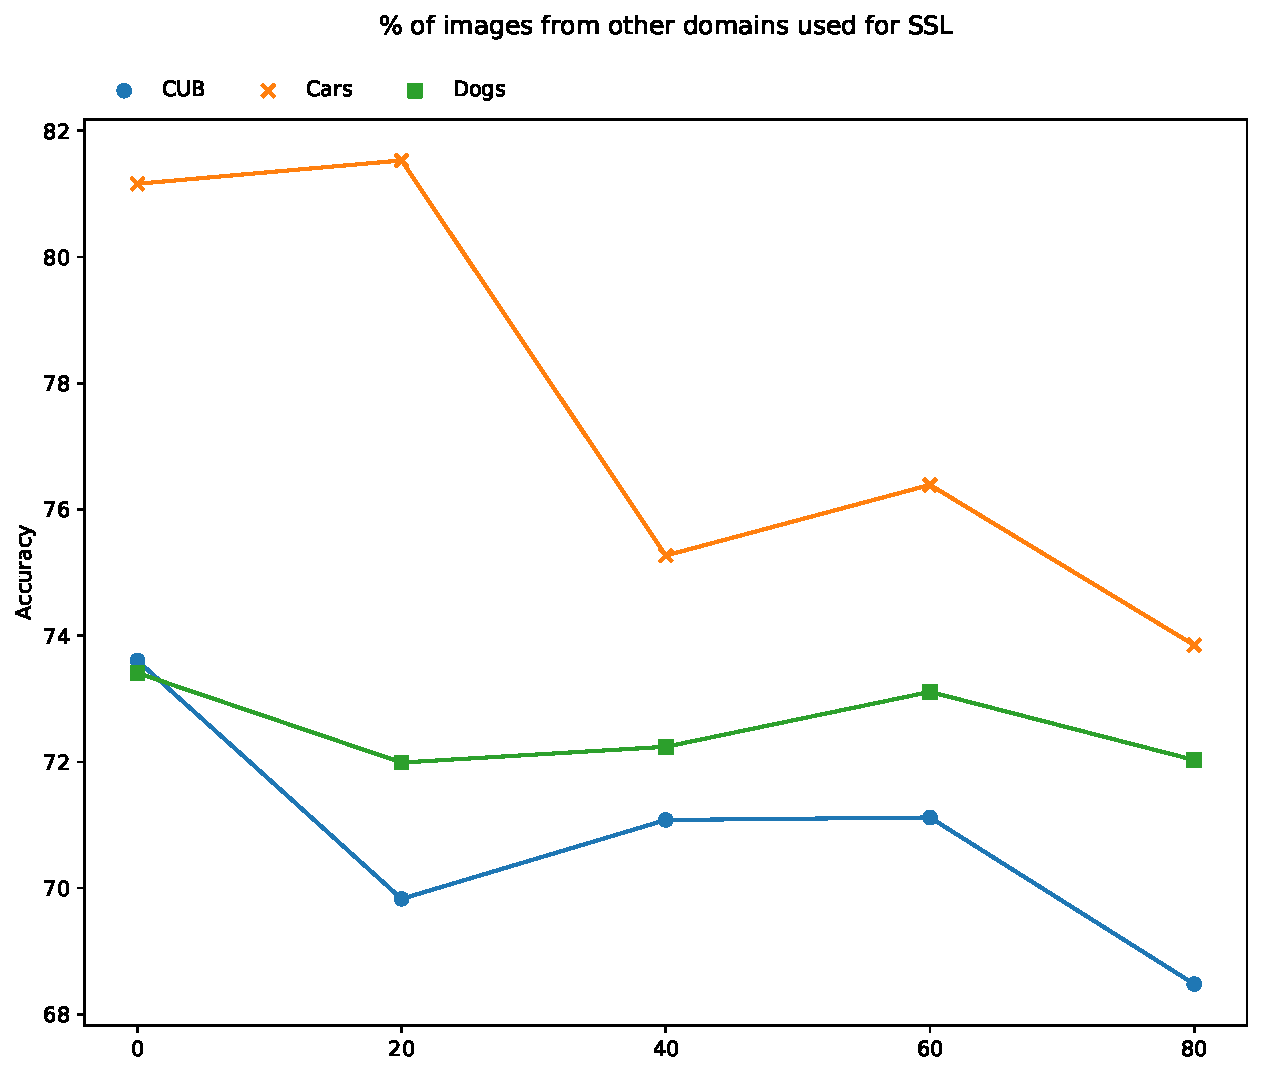
\includegraphics[width=5cm, height=5.5cm]{pdfs/ssl_other_domains.pdf} % first figure itself
        \caption{Performance on tasks \\ where a portion of the labelled data \\ is replaced with data from \\ other domains}
        \label{fig:20-60-other}
    \end{minipage}\hfill
    \begin{minipage}{0.33\textwidth}
        % \centering
        \includegraphics[width=6cm, height=4.5cm]{pdfs/grey_low_res.pdf} % first figure itself
        \caption{Results of applying self-supervised learning on artificially constructed harder tasks.}
        \label{fig:lowres}
    \end{minipage}\hfill
\end{figure}

\subsubsection{Unlabelled data for SSL from dissimilar domains negatively impacts the few-shot learner}

Verifying claim $3$ of the paper, we replace a portion of the labelled data, starting from 20\% of the data to 80\% of the data, with data from other domains. Here, we combine the data from all other datasets together, and sample images at random. We present results on $3$ chosen datasets, again, to save computation and time for other results. Results are given in figure \ref{fig:20-60-other} and table \ref{table:20_ssl_others} (appendix). The claim that using data from dissimilar domains for self-supervision is detrimental to few-shot classification holds true.

% \begin{figure*}[hbt!]
%     \centering
%     \begin{minipage}{0.9\textwidth}
%         \centering
%         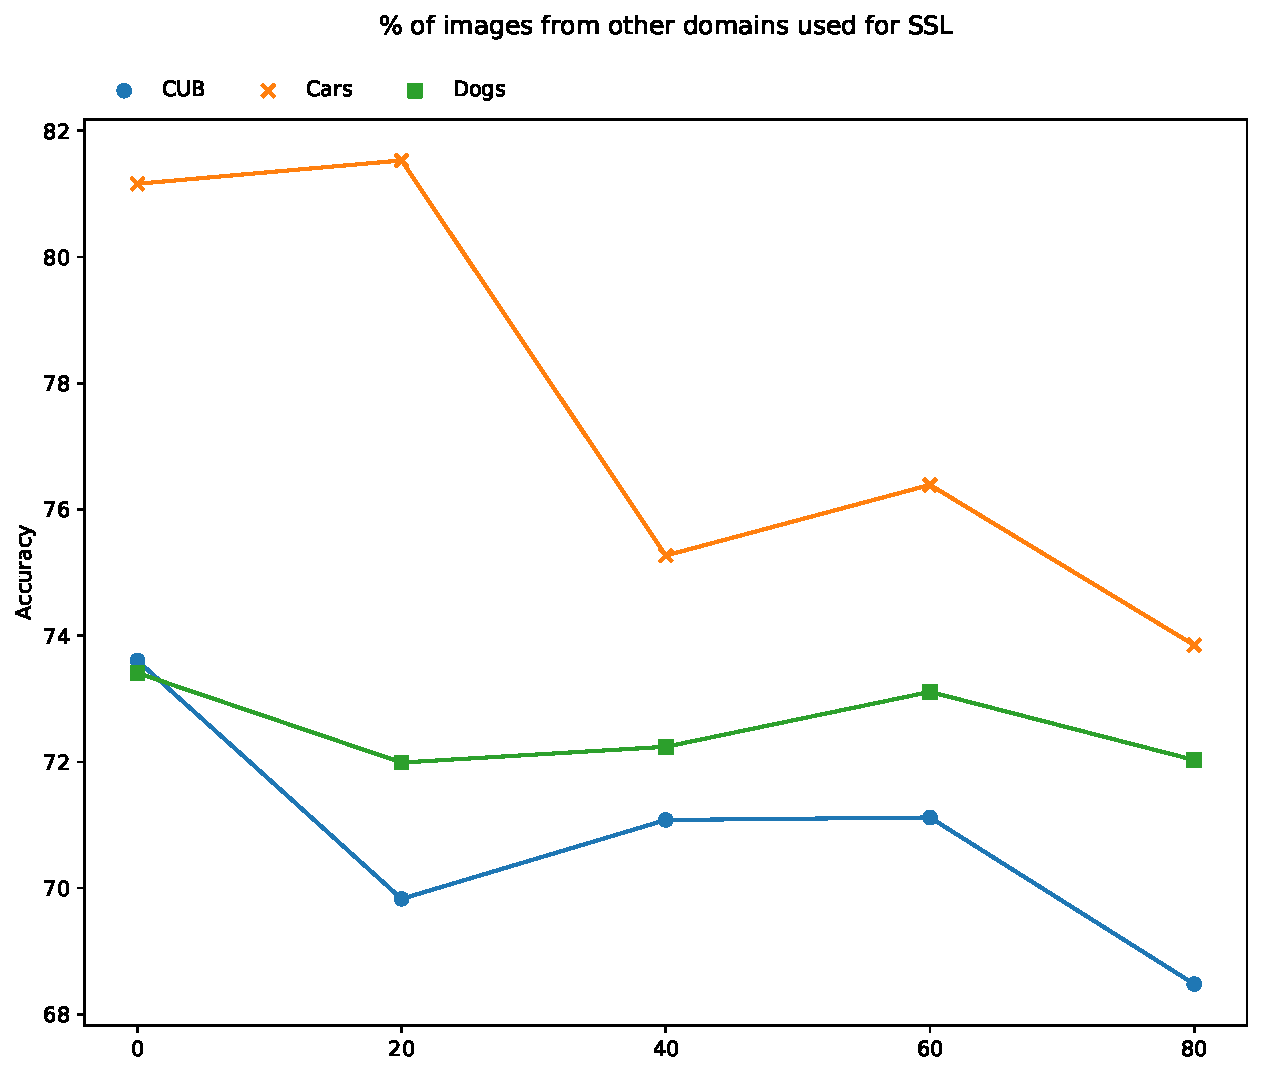
\includegraphics[width=0.8\textwidth, height=8.5cm]{pdfs/ssl_other_domains.pdf} % first figure itself
%         \caption{Performance on tasks where a portion of the labelled data is replaced with data from other domains}
%         \label{fig:20-60-other}
%     \end{minipage}\hfill
% \end{figure*}


\subsubsection{The proposed domain selection algorithm can alleviate this issue by learning to pick images from a large and generic pool of images}

To verify claim $4$, we implement the domain selection algorithm from scratch, and verify it across all $5$ small datasets as given in the paper, to make sure that we have got the implementation right. Results are presented in figure \ref{fig:domain} and table \ref{table:domain} in the appendix. Results are shown on using only 20\% of the labelled data for learning, only selecting images from other domains at random, and on using the proposed domain selection algorithm. We successfully verify and demonstrate that the algorithm proposed by the authors for selecting images from multiple dissimilar domains.

% \begin{figure*}[hbt!]
%     \centering
    
% \end{figure*}

\subsection{Results beyond original paper}

\label{subsubsec:conv4}
\subsubsection{Results on a different architecture - Conv4}

Here, we aim to investigate whether the claims of the paper hold when a small architecture that needs a smaller image size (84x84) is used. In particular, we investigate claim $1$ of the paper extensively. Note that the authors do not report results with this architecture. Results are given in figure \ref{fig:Conv4}. Exact numbers are given in tables \ref{table:conv_few_shot} and \ref{table:mini_imagenet_both} in the appendix. We find that the results \textbf{do not hold true} when a smaller architecture and image size is used, and that claim depends heavily on the architecture and image size. We present results across all the $5$ small datasets for completeness, across both SSL tasks. To confirm our claims, we also rerun results with another seed, but get similar results (Table \ref{table:seed_conv} in appendix).  

We next study the effect of $\alpha$ on the results, with the CUB and cars datasets in tables \ref{table:conv_rotation} and \ref{table:conv_jigsaw}. Here we find that the value of $\alpha$ plays an important role in the performance, and that high values leading to too much self-supervision is detrimental when the model is small. Even across training and testing with multiple $\alpha$ values, we find that the self-supervision provides only a marginal boost in $1$ out of $4$ cases, invalidating claim $1$ of the paper that self-supervision provides a stable boost to few-shot learners.

% \begin{figure*}[hbt!]
%     \centering
    
% \end{figure*}

\begin{table}
\parbox{.45\linewidth}{
    \centering
    \begin{tabular}{|c|c|c|}
            \hline
            Rotation & CUB & Cars \\
            \hline\hline
            $\alpha = 0$ (no SSL) & \textbf{77.72 \textpm\ 0.71} & \textbf{67.6 \textpm\ 0.84} \\
            $\alpha = 0.1$ & 77.6 \textpm\ 0.73 & 66.83 \textpm\ 0.75 \\
            $\alpha = 0.3$ & 77.22 \textpm\ 0.9 & 65.53 \textpm\ 0.73 \\
            $\alpha = 0.5$ & 74.57 \textpm\ 0.81 &66.61 \textpm\ 0.73 \\
            
            \hline
        \end{tabular}
    \caption{Conv-4's performance on applying SSL through Rotation}
    \label{table:conv_rotation}    
    }
    \hfill
    \parbox{.45\linewidth}{
    \centering
    \begin{tabular}{|c|c|c|}
            \hline
            Jigsaw & CUB & Cars \\
            \hline\hline
            $\alpha = 0$ (no SSL) & \textbf{77.72 \textpm\ 0.71} & \textbf{67.6 \textpm\ 0.84} \\
            $\alpha = 0.1$ & 75.57 \textpm\ 0.73 & 62.548 \textpm\ 0.75 \\
            $\alpha = 0.3$ & 64.91 \textpm\ 0.9 & 51.83 \textpm\ 0.73 \\
            $\alpha = 0.5$ & 69.09 \textpm\ 0.81 &60.39 \textpm\ 0.73 \\
            
            \hline
        \end{tabular}
    \caption{Conv-4's performance on applying SSL through Jigsaw}
    \label{table:conv_jigsaw}
    }
\end{table} 

 

% \begin{tabular}{cc}
%     \begin{minipage}{.5\linewidth}
        
%     \end{minipage} &

%     \begin{minipage}{.5\linewidth}
        
%     \end{minipage} 
% \end{tabular} 

% \begin{table*}[hbt!]
% \begin{center}
% \end{center}
% \caption{Conv-4's performance on Rotation.}
% \label{table:conv_rotation}
% \end{table*}

% \begin{table*}[hbt!]
% \begin{center}

% \end{center}
% \caption{Conv-4's performance on Jigsaw.}
% \label{table:conv_jigsaw}
% \end{table*}

\subsubsection{Results on cross-domain few-shot learning}

In another effort to extend the paper's results, we test the results of our trained models on the BSCD-FSL benchmark for cross-domain few-shot learning, introduced by \cite{guo2020broader} with their code \footnote[7]{\url{https://github.com/IBM/cdfsl-benchmark}}. The benchmark requires ImageNet-based trained few-shot models to evaluated on four cross-domain datasets: CropDiseases, EuroSAT, ISIC2018, and ChestX datasets, which covers plant disease images, satellite images, dermoscopic images of skin lesions, and X-ray images, respectively. The selected datasets reflect real-world use cases for few-shot learning since collecting enough examples from above domains is often difficult, expensive, or in some cases not possible. We use this benchmark to find out if models trained with self-supervision provide gains over normal supervised models when tested  on \textit{real-world datasets}. We test our mini-ImageNet trained models on this benchmark, to find out if self-supervision improves results on cross-domain datasets. Results on the ResNet-18 models are reported in table \ref{table:cdfsl_resnet}. Results on the Conv-4 models are given in appendix table \ref{table:cdfsl_conv}. 
We find that self-supervision results in learning heavily domain-specific representations, and that the results of the fully-supervised learner are much better than those with auxiliary tasks as self-supervision.


\begin{figure}[t]
    \begin{minipage}{0.5\textwidth}
        \centering
        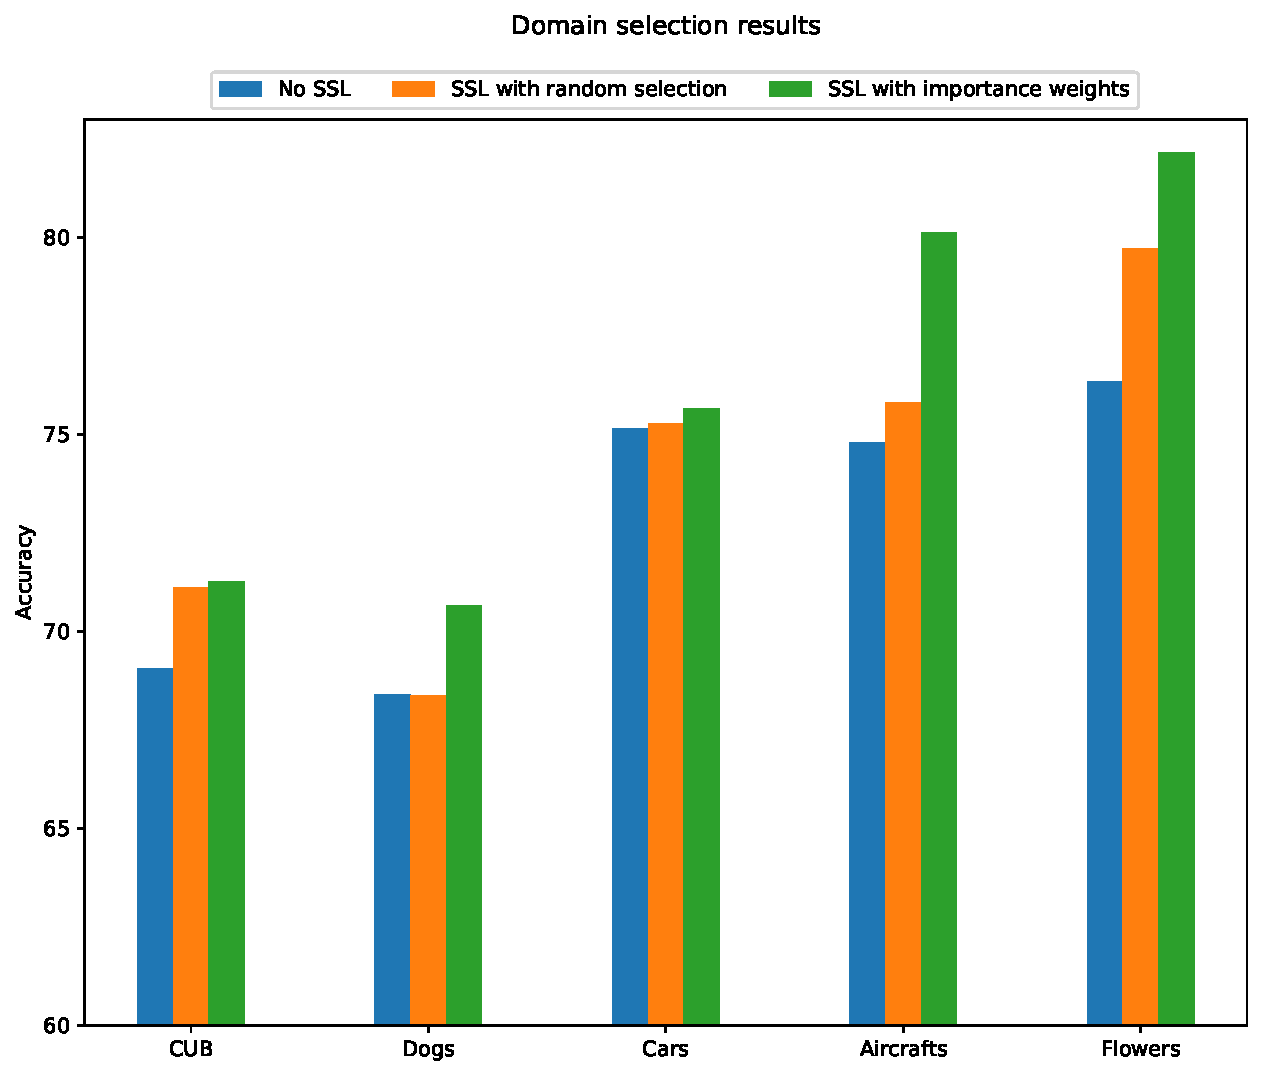
\includegraphics[, height=7cm]{pdfs/domain.pdf} % first figure itself
        \caption{Results of the domain selection algorithm}
        \label{fig:domain}
    \end{minipage}\hfill
    \begin{minipage}{0.5\textwidth}
        \centering
        \includegraphics[ height=7cm]{pdfs/Conv4.pdf} % first figure itself
        \caption{Results of using SSL with the Conv4 architecture}
        \label{fig:Conv4}
    \end{minipage}\hfill
\end{figure}

\begin{table*}[hbt!]
\begin{center}
\begin{tabular}{|c|c|c|c|c|}
\hline
Method & ChestX & Crop Disease & EuroSAT & ISIC \\
\hline\hline
ProtoNet & \textbf{24.32 \textpm\ 0.41} & \textbf{83.36 \textpm\ 0.63} & \textbf{76.09 \textpm\ 0.74} & 41.60 \textpm\ 0.58 \\
ProtoNet + Jigsaw & 23.97 \textpm\ 0.39 & 77.86 \textpm\ 0.69 & 72.72 \textpm\ 0.68 & 41.22 \textpm\ 0.56 \\
ProtoNet + Rotation & 23.84 \textpm\ 0.39 & 79.11 \textpm\ 0.68 & 72.47 \textpm\ 0.69 & \textbf{43.79 \textpm\ 0.61} \\
ProtoNet + Jigsaw + Rotation & 23.73 \textpm\ 0.38 & 77.39 \textpm\ 0.68 & 71.91 \textpm\ 0.7 & 40.05 \textpm\ 0.55 \\

\hline
\end{tabular}
\end{center}
\caption{CDFSL Benchmark for ResNet-18}
\label{table:cdfsl_resnet}
\end{table*}


\section{Discussion}

We find that the \textbf{central claims of the author as given in Section \ref{sec:claims} hold true, when the same architecture is used}. Considering the ResNet-18 model used in the paper with an input image size of 224, we find that self-supervision - in particular the jigsaw task, provides a boost in the case of small datasets. Experimentally, we verify claim $1$ of the paper on all small datasets and miniImageNet. However, going beyond the paper's architecture, we find that the results depend heavily on the image size and architecture and do not give the same gains with Conv-4-64, another architecture common in the few-shot learning literature, with an input image size of 84. Further ablation reveals that the jigsaw task in particular has a strong influence in this setup, and the rotation task requires tuning the $\alpha$ parameter to even reach the accuracy of the fully-supervised model. Future work may investigate ways to boost the performance of few-shot classifiers when the input sizes are small, and may also find out better architectures to use when the input size is small. Future work may also experiment with other available architectures, and find out if self-supervision increases performances across all configurations.

Regarding claims $2$ and $3$ such as on harder tasks and scenarios with lesser labelled data in the base dataset, our experiments on selected datasets verify that the claims hold true, with the ResNet-18 backbone. Further, we verify claim $4$ of the paper by implementing the domain selection algorithm from scratch and our experiments on all the 5 datasets show that relative gains are achieved. Future work may also investigate if the same claims hold true when different architectures were used. 

Finally, we evaluate the miniImageNet-trained models on a more practical setting of cross-domain few-shot learning and find that SSL during the training time does not help few-shot learners generalize across domains better. Future work may investigate why applying SSL results in domain-specific features, and propose methods to apply SSL in a more domain-agnostic manner.  We recommend future works in few-shot learning to train and evaluate in multiple architectures with different resolutions and verify their work more thoroughly.

\subsection{Communication with original authors}

We maintained communication with the authors throughout our implementation and training phase, spanning two months. We were able to clarify many implementation details in the original codebase, and the authors also re-ran an experiment on their side to test if the numbers match. Further, we received a lot of help regarding implementation of the domain selection algorithm, and could also confirm the implementation with them. We acknowledge and thank the authors for their help with the reproducibility of their paper.

\section{Acknowledgements}

The authors are grateful to \href{https://wandb.ai/}{Weights \& Biases} and \href{https://dagshub.com/}{DAGsHub} for reproducibility grants that supported this work.

\newpage